\documentclass[a4paper, final]{article}
\usepackage{cmap}
%\usepackage{literat} % Нормальные шрифты
\usepackage[14pt]{extsizes} % для того чтобы задать нестандартный 14-ый размер шрифта
\usepackage[T2A]{fontenc}
\usepackage[UTF8]{inputenc}
\usepackage[russian]{babel}
\usepackage{listings} %листинги
\usepackage{amsmath}
\usepackage{amssymb} % Для красивого значка пустого множества
\usepackage[left=25mm, top=20mm, right=20mm, bottom=20mm, footskip=10mm]{geometry}
\usepackage{ragged2e} %для растягивания по ширине
\usepackage{setspace} %для межстрочного интервала
\usepackage{indentfirst} % для абзацного отступа
\usepackage{moreverb} %для печати в листинге исходного кода программ
\renewcommand\verbatimtabsize{4\relax}
\renewcommand\listingoffset{0.2em} %отступ от номеров строк в листинге
\renewcommand{\arraystretch}{1.4} % изменяю высоту строки в таблице
\usepackage[font=small, singlelinecheck=false, justification=centering, format=plain, labelsep=period]{caption} %для настройки заголовка таблицы
\usepackage{listingsutf8}
\usepackage{xcolor} % цвета
\usepackage{hyperref}% для гиперссылок
\usepackage{enumitem} %для перечислений
\usepackage{titlesec}
\usepackage{graphicx}
\graphicspath{ {./Рисунки/} }
%\usepackage{float}
\usepackage{booktabs}
\usepackage{floatrow}
\usepackage{scalerel} % Stretching images
\usepackage[final]{pdfpages}
\usepackage{multirow}
\usepackage{array}
\usepackage{tabularx}

\definecolor{apricot}{HTML}{FFF0DA}
\definecolor{mygreen}{rgb}{0,0.6,0}
\definecolor{string}{HTML}{B40000} % цвет строк в коде
\definecolor{comment}{HTML}{008000} % цвет комментариев в коде
\definecolor{keyword}{HTML}{1A00FF} % цвет ключевых слов в коде
\definecolor{morecomment}{HTML}{8000FF} % цвет include и других элементов в коде
\definecolor{captiontext}{HTML}{FFFFFF} % цвет текста заголовка в коде
\definecolor{captionbk}{HTML}{999999} % цвет фона заголовка в коде
\definecolor{bk}{HTML}{FFFFFF} % цвет фона в коде
\definecolor{frame}{HTML}{999999} % цвет рамки в коде
\definecolor{brackets}{HTML}{B40000} % цвет скобок в коде





\AtBeginDocument{\renewcommand{\contentsname}{Содержание}}
\AtBeginDocument{\renewcommand{\refname}{Список источников}}
% Настраиваем листинги, чтобы они использовали счётчик figure
\AtBeginDocument{
  \renewcommand{\thelstlisting}{\thefigure}  % Листинги используют тот же счетчик, что и рисунки
  \renewcommand{\lstlistingname}{Рис.}    % Меняем подпись
}

% Автоматически увеличиваем счетчик figure перед каждым листингом
\let\oldlstlisting\lstlisting
\renewcommand{\lstlisting}[1][]{%
    \refstepcounter{figure}% Увеличиваем счетчик figure
    \oldlstlisting[#1]% Вызываем оригинальную команду lstlisting
}
\lstset{
    captionpos=b
}
\newcommand{\specialcell}[2][l]{\begin{tabular}[#1]{@{}l@{}}#2\end{tabular}} % Алиас для таблиц

\floatsetup[table]{style=plain,capposition=top} % Подпись таблицы сверху
\setlist[enumerate,itemize]{leftmargin=1.2cm} %отступ в перечислениях

\hypersetup{colorlinks,
  allcolors=[RGB]{000 000 000}} %красивые гиперссылки (не красные)

% подгружаемые языки — подробнее в документации listings (это всё для листингов)
\lstloadlanguages{ [LaTeX] TeX}
% включаем кириллицу и добавляем кое−какие опции
\lstset{language =[LaTeX] TeX, % выбираем язык по умолчанию
extendedchars=true , % включаем не латиницу
escapechar = | , % |«выпадаем» в LATEX|
frame=tb , % рамка сверху и снизу
commentstyle=\itshape , % шрифт для комментариев
stringstyle =\bfseries} % шрифт для строк

\textheight=24cm % высота текста
\textwidth=16cm % ширина текста
\oddsidemargin=0pt % отступ от левого края
\topmargin=-1.5cm % отступ от верхнего края
\parindent=24pt % абзацный отступ
\parskip=0pt % интервал между абзацами
\tolerance=2000 % терпимость к "жидким" строкам
\flushbottom % выравнивание высоты страниц

\begin{document} % начало документа
\setcounter{tocdepth}{2} % Вложенность не больше 2 в содержании
\lstset{
  language=haskell, % Язык кода по умолчанию
  morekeywords={*,...}, % если хотите добавить ключевые слова, то добавляйте
  % Цвета
  keywordstyle=\color{keyword}\ttfamily\bfseries,
  %stringstyle=\color{string}\ttfamily,
  stringstyle=\ttfamily\color{red!50!brown},
  commentstyle=\color{comment}\ttfamily,
  morecomment=[l][\color{morecomment}]{\#},
  % Настройки отображения
  breaklines=true, % Перенос длинных строк
  basicstyle=\ttfamily\footnotesize, % Шрифт для отображения кода
  backgroundcolor=\color{bk}, % Цвет фона кода
  frame=single,xleftmargin=\fboxsep,xrightmargin=-\fboxsep, % Рамка, подогнанная к заголовку
  rulecolor=\color{frame}, % Цвет рамки
  tabsize=3, % Размер табуляции в пробелах
  % Настройка отображения номеров строк. Если не нужно, то удалите весь блок
  numbers=left, % Слева отображаются номера строк
  stepnumber=1, % Каждую строку нумеровать
  numbersep=5pt, % Отступ от кода
  numberstyle=\small\color{black}, % Стиль написания номеров строк
  % Для отображения русского языка
  extendedchars=true,
  literate={Ö}{ {\"O} }1
  {~}{ {\textasciitilde} }1
  {а}{ {\selectfont\char224} }1
  {б}{ {\selectfont\char225} }1
  {в}{ {\selectfont\char226} }1
  {г}{ {\selectfont\char227} }1
  {д}{ {\selectfont\char228} }1
  {е}{ {\selectfont\char229} }1
  {ё}{ {\"e} }1
  {ж}{ {\selectfont\char230} }1
  {з}{ {\selectfont\char231} }1
  {и}{ {\selectfont\char232} }1
  {й}{ {\selectfont\char233} }1
  {к}{ {\selectfont\char234} }1
  {л}{ {\selectfont\char235} }1
  {м}{ {\selectfont\char236} }1
  {н}{ {\selectfont\char237} }1
  {о}{ {\selectfont\char238} }1
  {п}{ {\selectfont\char239} }1
  {р}{ {\selectfont\char240} }1
  {с}{ {\selectfont\char241} }1
  {т}{ {\selectfont\char242} }1
  {у}{ {\selectfont\char243} }1
  {ф}{ {\selectfont\char244} }1
  {х}{ {\selectfont\char245} }1
  {ц}{ {\selectfont\char246} }1
  {ч}{ {\selectfont\char247} }1
  {ш}{ {\selectfont\char248} }1
  {щ}{ {\selectfont\char249} }1
  {ъ}{ {\selectfont\char250} }1
  {ы}{ {\selectfont\char251} }1
  {ь}{ {\selectfont\char252} }1
  {э}{ {\selectfont\char253} }1
  {ю}{ {\selectfont\char254} }1
  {я}{ {\selectfont\char255} }1
  {А}{ {\selectfont\char192} }1
  {Б}{ {\selectfont\char193} }1
  {В}{ {\selectfont\char194} }1
  {Г}{ {\selectfont\char195} }1
  {Д}{ {\selectfont\char196} }1
  {Е}{ {\selectfont\char197} }1
  {Ё}{ {\"E} }1
  {Ж}{ {\selectfont\char198} }1
  {З}{ {\selectfont\char199} }1
  {И}{ {\selectfont\char200} }1
  {Й}{ {\selectfont\char201} }1
  {К}{ {\selectfont\char202} }1
  {Л}{ {\selectfont\char203} }1
  {М}{ {\selectfont\char204} }1
  {Н}{ {\selectfont\char205} }1
  {О}{ {\selectfont\char206} }1
  {П}{ {\selectfont\char207} }1
  {Р}{ {\selectfont\char208} }1
  {С}{ {\selectfont\char209} }1
  {Т}{ {\selectfont\char210} }1
  {У}{ {\selectfont\char211} }1
  {Ф}{ {\selectfont\char212} }1
  {Х}{ {\selectfont\char213} }1
  {Ц}{ {\selectfont\char214} }1
  {Ч}{ {\selectfont\char215} }1
  {Ш}{ {\selectfont\char216} }1
  {Щ}{ {\selectfont\char217} }1
  {Ъ}{ {\selectfont\char218} }1
  {Ы}{ {\selectfont\char219} }1
  {Ь}{ {\selectfont\char220} }1
  {Э}{ {\selectfont\char221} }1
  {Ю}{ {\selectfont\char222} }1
  {Я}{ {\selectfont\char223} }1
  {\{}{ { {\color{brackets}\{} } }1 % Цвет скобок {
  {\} }{ { {\color{brackets}\} } } }1 % Цвет скобок }
}

% НАЧАЛО ТИТУЛЬНОГО ЛИСТА
\begin{center}
\hfill \break
\hfill \break
\normalsize{МИНИСТЕРСТВО НАУКИ И ВЫСШЕГО ОБРАЗОВАНИЯ РОССИЙСКОЙ ФЕДЕРАЦИИ\\
 федеральное государственное автономное образовательное учреждение высшего образования «Санкт-Петербургский политехнический университет Петра Великого»\\[5pt]}
\normalsize{Институт компьютерных наук и кибербезопасности}\\[5pt] 
\normalsize{Высшая школа технологий искусственного интеллекта}\\[5pt] 
\normalsize{Направление: 02.03.01 Математика и компьютерные науки}\\

\hfill \break
\hfill \break
\hfill \break
\large{Отчёт по дисциплине}\\
\large{<<Образовательный форсайт>>}\\
\hfill \break
\large{<<Наука о данных и аналитика больших объемов данных>>}
\hfill \break
\hfill \break
\end{center}
 
\small{ 
\begin{tabular}{lrrl}
\!\!\!Студент, & \hspace{2cm} & & \\
\!\!\!группы 5130201/20102 & \hspace{2cm} & \underline{\hspace{3cm}} &Гаар В.С. \\\\
\!\!\!Преподаватель, \hspace{2cm} & & \\
\!\!\!к.т.н., доц. & \hspace{2cm} & \underline{\hspace{3cm}} &  Курочкин М.А. \\\\
&&\hspace{5cm}
\end{tabular}
\begin{flushright}
<<\underline{\hspace{1cm}}>>\underline{\hspace{2.5cm}} 2024 г.
\end{flushright}
}

\hfill \break
\hfill \break
\begin{center} \small{Санкт-Петербург, 2024} \end{center}
\thispagestyle{empty} % выключаем отображение номера для этой страницы

% КОНЕЦ ТИТУЛЬНОГО ЛИСТА
\newpage

\tableofcontents

\newpage

\cleardoublepage
\phantomsection
\addcontentsline{toc}{section}{Введение}
\section*{Введение}
В современных условиях работы с большими объемами данных стали неотъемлемой частью практически всех отраслей экономики. Обработка данных больших масштабов требует использования специализированных инструментов и подходов. Курс ''Наука о данных и аналитика больших объемов данных'' охватывает ключевые аспекты работы с данными, начиная от основ анализа данных и заканчивая современными методами обработки текстов.

Цель курса — сформировать системные знания и практические навыки анализа данных, которые можно применять в разнообразных профессиональных контекстах, включая бизнес, науку и технологии.

\newpage
\section{Постановка задачи}
В рамках курса <<Образовательный форсайт>> было необходимо пройти онлайн-курс <<Наука о данных и аналитика больших объемов данных>> на портале <<Открытое образование>> (\url{https://openedu.ru/}).

Задачей курса является предоставление учащимся комплексного представления о том, как анализировать данные, начиная от их подготовки и заканчивая визуализацией и интерпретацией результатов. В рамках курса:
\begin{itemize}
  \item Изучался жизненный цикл аналитики данных, от сбора и очистки данных до формирования бизнес-инсайтов.
  \item Осваивались технологии обработки больших данных, включая Hadoop и MapReduce.
  \item Осуществлялась работа с инструментами визуализации и анализа текстовой информации.
\end{itemize}

На протяжении курса выполнялись задания, направленные на практическое закрепление материала, и прошли итоговый тест для оценки уровня усвоения знаний.

\newpage
\section{Аннотация курса и разделов}
Курс состоит из семи тематических модулей:
\begin{enumerate}
  \item \textbf{Введение в большие данные} \\
На первом этапе курса учащиеся познакомились с основными концепциями и терминами, связанными с большими данными. Рассматривались основные характеристики больших данных (объем, скорость, разнообразие, достоверность и ценность) и их влияние на принятие решений.

  \item \textbf{Жизненный цикл аналитики данных} \\
Учащиеся изучали процесс анализа данных на уровне компаний, включая этапы консолидации, трансформации и загрузки данных (ETL). Особое внимание уделялось задачам интеграции данных из различных источников и проблемам обеспечения их качества.

  \item \textbf{Высокопроизводительные вычисления}\\
Этот модуль был посвящен использованию платформы Hadoop для распределенной обработки данных. Рассматривались история развития технологии, структура Hadoop Distributed File System (HDFS), и процесс MapReduce, обеспечивающий параллельное выполнение задач.

  \item \textbf{Масштабирование и многоуровневое хранение данных}\\
На этом этапе слушатели познакомились с основными принципами горизонтального и вертикального масштабирования, а также изучили подходы к репликации и шардингу данных. Особое внимание было уделено CAP-теореме и ее применению в распределенных системах.

  \item \textbf{Визуализация данных}\\
Рассматривались способы представления данных в виде графиков, диаграмм и инфографики. Учащиеся узнали, как с помощью визуализации можно ускорить процесс принятия решений и выявить скрытые закономерности в данных.

  \item \textbf{Статистические методы анализа данных}\\
Изучались основные статистические подходы, включая проверку гипотез и построение моделей. Учащиеся освоили критерии значимости и регрессии, а также познакомились с параметрическими и непараметрическими методами.

  \item \textbf{Анализ текстов}\\
Этот модуль был посвящен обработке неструктурированных данных. Учащиеся изучили методы анализа текстов, включая извлечение информации, анализ настроений и работу с текстовыми массивами данных.
\end{enumerate}

\newpage
\section{Теоретическая часть курса}
В рамках курса ''Наука о данных и аналитика больших объемов данных'' рассматривались ключевые темы, связанные с анализом больших данных, их обработкой и визуализацией. В теоретической части курса изучались следующие модули:
\begin{enumerate}
  \item \textbf{Введение в большие данные}\\
Основные концепции больших данных включали характеристики 3V (объем, скорость, разнообразие), дополненные признаками достоверности и ценности. Рассматривались причины возникновения больших данных, включая развитие технологий и увеличение объемов цифровой информации. Учащиеся узнали о важности использования специальных инструментов, таких как распределенные системы обработки, и о ключевых вызовах работы с большими данными, таких как интеграция и анализ разнородных источников данных

  \item \textbf{Жизненный цикл аналитики данных}\\
Этот модуль был посвящен процессам работы с данными в рамках полного жизненного цикла. Рассматривались следующие этапы:
    \begin{itemize}
      \item \textbf{Сбор данных:} объединение информации из разнородных источников.
      \item \textbf{Очистка данных:} устранение ошибок, пропусков и дубликатов.
      \item \textbf{Трансформация и агрегирование:} создание однородных структур для последующего анализа.
      \item \textbf{Загрузка и анализ:} использование ETL-процессов и бизнес-аналитики для принятия решений. Ключевой акцент был сделан на проблемах низкого качества данных и способах их решения, таких как использование стандартизированных форматов и инструментов обработки.
    \end{itemize}

  \item \textbf{Высокопроизводительные вычисления}\\
Этот модуль рассматривал технологии Hadoop и MapReduce как основу для распределенной обработки данных. Участники узнали о ключевых преимуществах платформы Hadoop:
    \begin{itemize}
      \item \textbf{Масштабируемость:} возможность увеличивать вычислительные мощности через добавление узлов.
      \item \textbf{Отказоустойчивость:} использование репликации данных для предотвращения потерь.
      \item \textbf{Эффективность:} параллельная обработка больших объемов данных. Изучалась архитектура Hadoop Distributed File System (HDFS), позволяющая обрабатывать данные размером от гигабайтов до петабайтов, и основы MapReduce для выполнения сложных аналитических задач.
    \end{itemize}

  \item \textbf{Масштабирование и многоуровневое хранение данных}\\
В рамках модуля рассматривались принципы горизонтального и вертикального масштабирования:
    \begin{itemize}
      \item \textbf{Горизонтальное масштабирование:} добавление новых узлов для повышения производительности.
      \item \textbf{Вертикальное масштабирование:} замена существующих компонентов на более мощные. Также изучались подходы репликации (Master-Slave и Peer-to-Peer) и шардинга для распределения нагрузки между серверами. Участники познакомились с CAP-теоремой, определяющей баланс между согласованностью данных, доступностью и устойчивостью к разделению в распределенных системах
    \end{itemize}

  \item \textbf{Визуализация данных}\\
Участники изучали важность визуального представления данных для анализа и принятия решений. Рассматривались основные инструменты визуализации, включая:
    \begin{itemize}
      \item \textbf{Графики и диаграммы:} точечные, линейные, столбчатые и круговые диаграммы.
      \item \textbf{Инфографика:} сочетание текстов, графиков и изображений для наглядного представления информации.
      \item \textbf{Дашборды:} интерактивные панели для мониторинга ключевых показателей. Изучались подходы к созданию визуализаций, отвечающих требованиям масштабируемости и интерпретации сложных структур данных 
    \end{itemize}

  \item \textbf{Статистические методы анализа данных}\\
Основное внимание было уделено анализу выборок и проверке гипотез. Рассматривались:
    \begin{itemize}
      \item \textbf{Параметрические методы:} t-критерий Стьюдента, критерий Фишера.
      \item \textbf{Непараметрические методы:} анализ рангов и частот.
      \item \textbf{Оценка параметров:} точечная и интервальная. Изучались ключевые понятия, такие как ошибки первого и второго рода, уровень значимости, и критерии согласия для оценки достоверности данных
    \end{itemize}

  \item \textbf{Анализ текстов}\\
Этот модуль был посвящен обработке неструктурированных данных. Рассматривались методы извлечения информации, включая:
    \begin{itemize}
      \item \textbf{Анализ настроений:} определение общего мнения на основе текстовых данных.
      \item \textbf{Категоризация и классификация текстов:} выделение ключевых тематических групп.
      \item \textbf{Text Mining:} применение методов Data Mining для анализа текстов. Особое внимание уделялось использованию текстовых данных для прогнозирования и выявления закономерностей
    \end{itemize}
\end{enumerate}
 

\newpage
\section{Результаты аттестации по модулям}
На Рис.~\ref{img:exam} представлены результаты прохождения итоговой аттестации.

\begin{figure}[H]
   \centering
   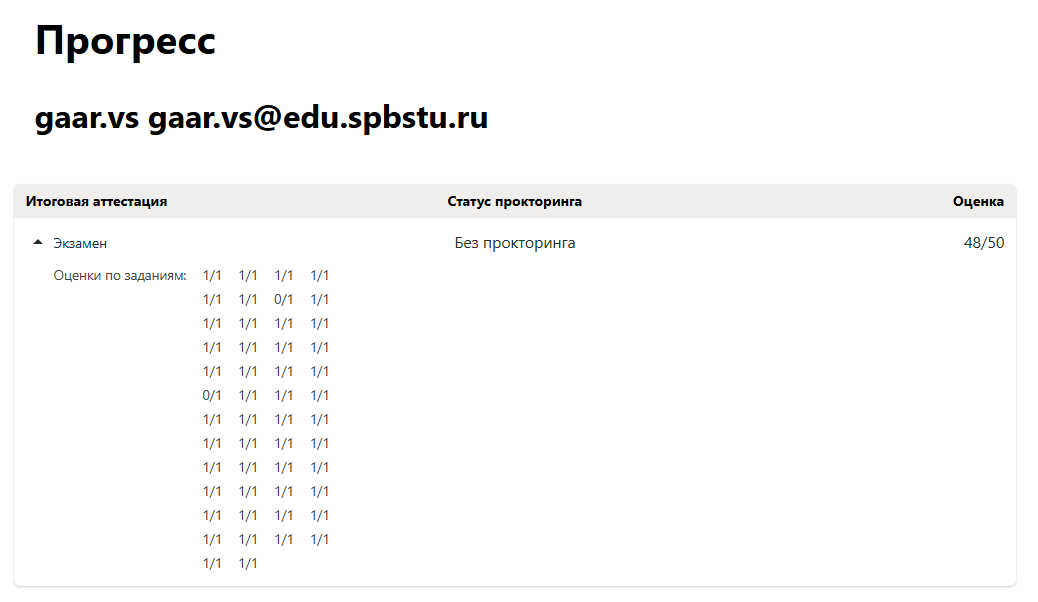
\includegraphics[width=1\linewidth]{exam.png}
   \caption{Результаты прохождения итоговой аттестации}
   \label{img:exam}
\end{figure}

Как видно, итоговый тест был пройден на 48/50 баллов, что соответствует оценке 96\% при проходном балле 50\%.

\cleardoublepage
\phantomsection
\newpage
\addcontentsline{toc}{section}{Заключение}
\section*{Заключение}
Пройдя курс ''Наука о данных и аналитика больших объемов данных'', я получил ценные знания и навыки, которые помогают лучше понимать и решать задачи обработки и анализа данных. Курс охватывал ключевые аспекты работы с данными, включая их сбор, очистку, анализ, визуализацию и текстовую обработку. Каждый из модулей предоставил структурированное понимание современных технологий, таких как Hadoop, NoSQL и методы Text Mining.

Особенно полезным было изучение жизненного цикла аналитики данных и принципов работы распределенных систем, что позволило понять подходы к обработке больших объемов информации. Модуль по визуализации подчеркнул важность представления результатов в наглядной форме, а статистические методы анализа данных дали инструменты для принятия обоснованных решений.

Курс имеет ряд значительных преимуществ: структурированность материала, актуальность рассматриваемых тем и знакомство с передовыми инструментами работы с данными. Однако, как и у любого онлайн-обучения, здесь не хватало взаимодействия с преподавателями и коллегами, а также большего количества практических заданий для закрепления теоретических знаний.

Несмотря на эти ограничения, курс стал важным шагом в моем профессиональном развитии. Полученные знания и навыки я планирую использовать в решении реальных задач анализа данных, что позволит принимать более обоснованные и точные решения.
\cleardoublepage
\phantomsection
\newpage
%Список источников
\begin{thebibliography}{0}
	\bibitem{bib:carpet}
	OpenEdu. Наука о данных и аналитика больших объемов данных [Электронный ресурс] URL: \url{https://apps.openedu.ru/learning/course/course-v1:spbstu+BIGDATA+fall_2024/home} (дата обращения 10.12.2024).
\end{thebibliography}
\addcontentsline{toc}{section}{Список источников}

\end{document}